\documentclass{ujarticle}

%どうもbeginpgfgraphicnamedがtexファイルの名前と同じだとエラーになるっぽい


\usepackage[dvipdfmx]{graphicx}
\usepackage{tikz}
\usepackage{amsmath}    % required for `\align*' (yatex added)
\pgfrealjobname{sublattice}


\begin{document}
 \begin{figure}[htb]
  \centering
  
 \beginpgfgraphicnamed{sub}
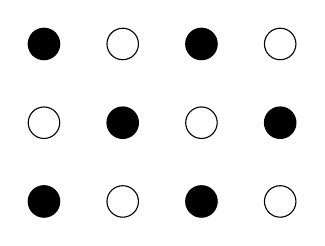
\begin{tikzpicture}
 %点の設定(sublattice A)
  \coordinate (A1) at (0,0);
  \coordinate (A2) at (2,0);
  \coordinate (A3) at (1,1);
  \coordinate (A4) at (3,1);
  \coordinate (A5) at (0,2);
  \coordinate (A6) at (2,2);

 
 %点の設定(sublattice B)
  \coordinate (B1) at (1,0);
  \coordinate (B2) at (3,0);
  \coordinate (B3) at (0,1);
  \coordinate (B4) at (2,1);
  \coordinate (B5) at (1,2);
  \coordinate (B6) at (3,2);

 
 %sublattice Aの描画
 \filldraw (A1) circle[radius=2mm];
 \filldraw (A2) circle[radius=2mm];
 \filldraw (A3) circle[radius=2mm];
 \filldraw (A4) circle[radius=2mm];
 \filldraw (A5) circle[radius=2mm];
 \filldraw (A6) circle[radius=2mm];

 
%sublattice Bの描画
 \filldraw[fill=white] (B1) circle[radius=2mm];
 \filldraw[fill=white] (B2) circle[radius=2mm];
 \filldraw[fill=white] (B3) circle[radius=2mm];
 \filldraw[fill=white] (B4) circle[radius=2mm];
 \filldraw[fill=white] (B5) circle[radius=2mm];
 \filldraw[fill=white] (B6) circle[radius=2mm];

% \fill[green, opacity=0.2]
%    (current bounding box.south west)
 %    rectangle (current bounding box.north east);
 
\end{tikzpicture}
  \endpgfgraphicnamed{sub}
 \end{figure}
 
\end{document}
